\jxhj{%教学后记
	}
\skrq{%授课日期
	2017年5月9日 4-5节}
\ktmq{%课题名称
	 极坐标指令}
\jxmb{%教学目标,每行前面要加 \item
	\item 掌握Fanuc上极坐标指令的使用;
	\item 掌握Siemens上极坐标指令的使用;
	\item 灵活使用极坐标指令进行编程;
	\item 掌握加工工艺的分析。 }
\jxzd{%教学重点,每行前面要加 \item
	\item 极坐标知识和其指令的使用;
	\item 对加工轮廓进行处理后再编程。 }
\jxnd{%教学难点,每行前面要加 \item
	\item 加工轮廓进行处理后再编程。 }
\jjff{%教学方法
	通过讲述、举例、演示法来说明;}

\makeshouye %制作教案首页

%%%%教学内容
\subsection{组织教学}
\begin{enumerate}[\hspace{2em}1、]
	\item 集中学生注意力;
	\item 清查学生人数;
	\item 维持课堂纪律;
\end{enumerate}
\subsection{复习导入及主要内容}
\begin{enumerate}[1、]
	\item 旋转可应用场合;
	\item 要素及原理;
	\item Fanuc旋转指令格式;
	\item Sienes旋转指令格式;
	\item 编程实例。
\end{enumerate}



\subsection{教学内容及过程}

\subsubsection{加工轮廓的处理}
\begin{figure}
	\centering	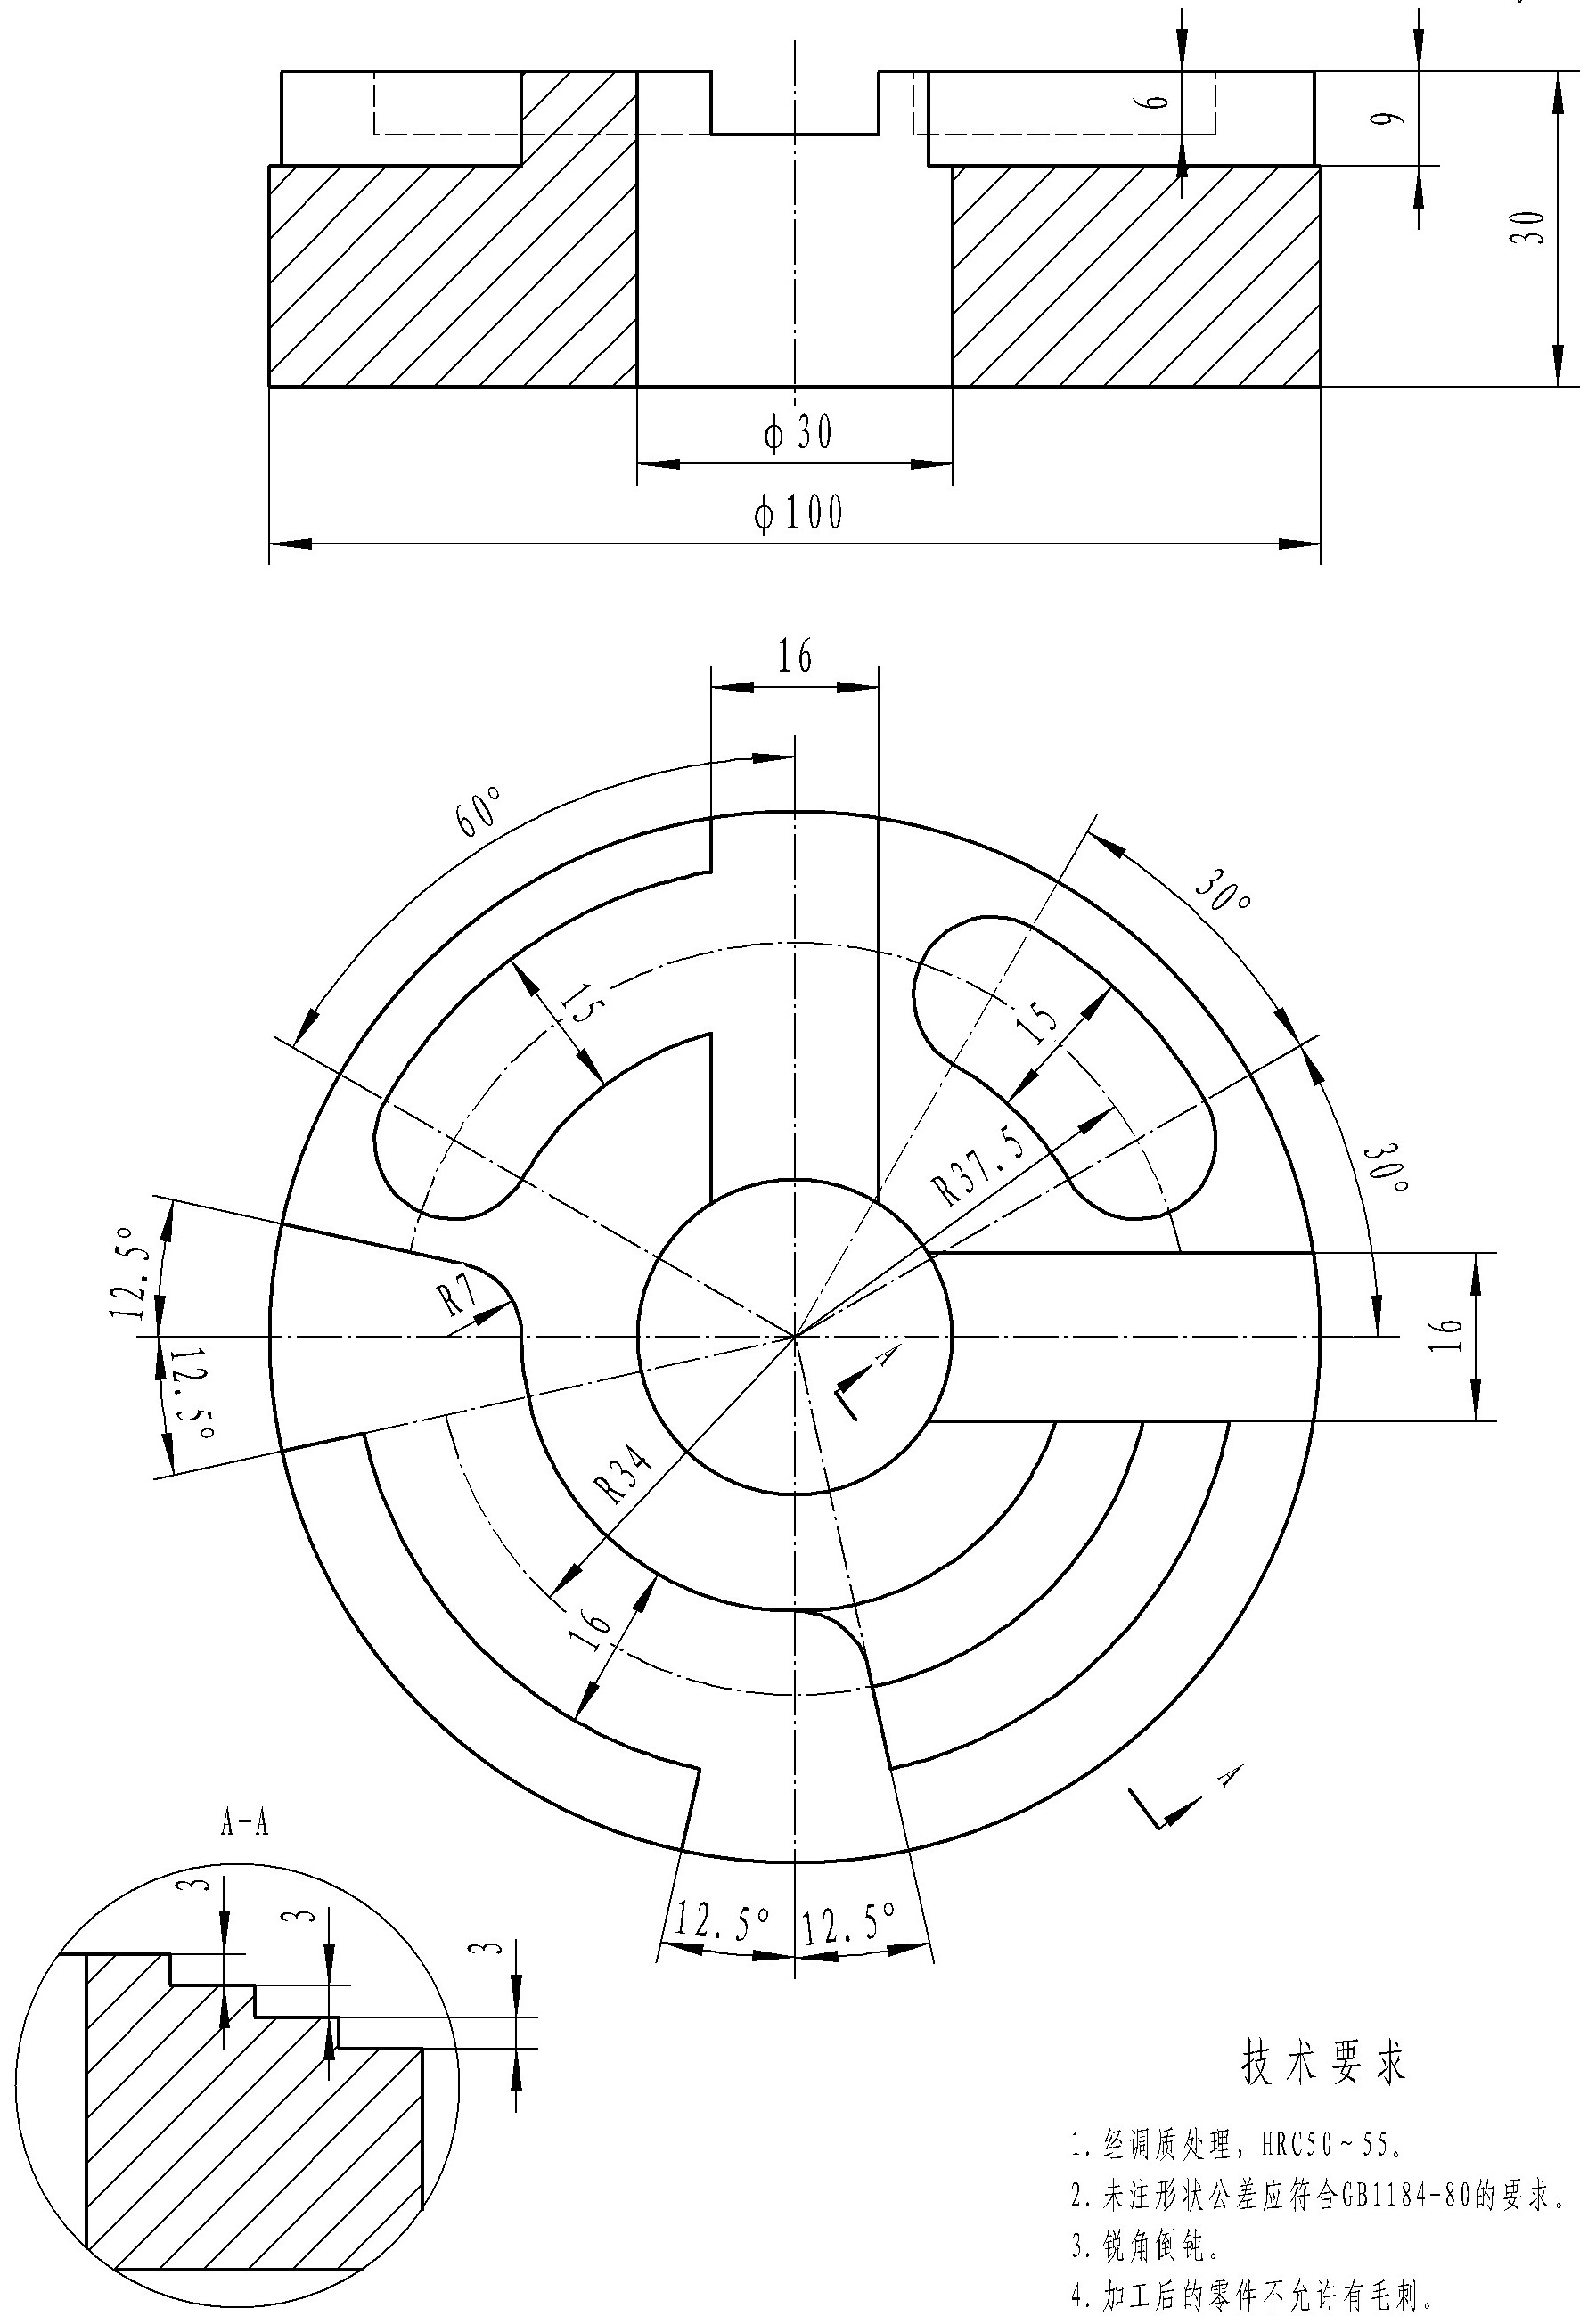
\includegraphics[width=0.8\textwidth]{images/9-1}
	\caption{极坐标实例} \label{极坐标实例}
\end{figure}
\textbf{加工轮廓的处理(改路径,延长)}
\paragraph{把加工轮廓进行拆分}
\noindent A、两个直槽:\\
标点的坐标,直角坐标(开放的)\\
B、小圆弧槽:\\
标点的坐标,使用极坐标\\
C、腰形槽:\\
标点的坐标,极坐标\\
D、扇形台阶\\
标点的坐标,极坐标\\
起点与终点不重合\\
编程时的处理\\
E、带翅膀的圆弧槽。
\paragraph{极坐标与 直角坐标的互换}
$$X=P*cosA$$
$$Y=P*sinA$$
$$P=X2+Y2$$
$$A=aictanY/X$$
\subsubsection{极坐标}
\paragraph{Fanuc上的极坐标}
指令格式: G\_\_ G~~ G16;启动极坐标指令(极坐标方式)\\
G~~ IP\_\_; 极坐标指令\\
:\\
G15;取消极坐标\\
说明:G\_\_极坐标指令的平面选择(G17、G18、G19)\\
G~~ G90指定工件坐标系的零点作为极坐标系原点,\\
G91指定当前位置作为极坐标系的原点。\\
IP\_\_指定极坐标系选择平面的轴地址及其值。\\
第1轴:极坐标半径\\
第2轴:极坐标角度 \\
用G90指定半径,极点设在工件坐标系原点。\\
如再用G90指定角度,角度是与X轴的夹角\\
如再用G91指定角度,角度是与当前位置的夹角\\
用G91指定半径,极点设在刀具当前位置。\\
如再用G90指定角度,角度是与X轴的夹角\\
如再用G91指定角度,角度是与当前位置的夹角。\\
限制:A、在极坐标方式中,对圆弧插补或螺旋线插补(G02,G03)用R 指定半径。\\
在极坐标方式中,不能用以下指令:\\
G4、G10、G52、G92、G53、G68、G51\\
在极坐标方式中不能倒角和倒圆\\
\paragraph{Siemens上的极坐标}
\textbf{极坐标,极点定义}:G110,G111,G112 \\
A、在直角坐标系中定义极点:\\
G110/G111/G112 X\_\_ Y\_\_ Z\_\_\\
B、在极坐标系中定义极点:\\
G110/G111/G112 AP=\_\_RP=\_\_\\
说明: \\
G110:相对于刀具最近到达的点(刀具当前位置)定义极点\\
G111:相对于当前工件坐标系定义极点\\
G112:相对于上一个有效极点定义极点\\
\textbf{在极坐标系中使用极坐标}\\
A、G0 AP=\_\_ RP=\_\_\\
B、G1 AP=\_\_ RP=\_\_\\
C、G2 AP=\_\_RP=\_\_\\
D、G3 AP=\_\_ RP=\_\_
说明:\\
AP=\_\_:极角,极点和目标点之间连线与角度参考方向之间的夹角(第一次角度参考方向线中一条),取值范围±(0-360),当用绝对坐标编程时,角度为相对于加工平面的水平轴方向,当用相对坐标编程时,上一个被编程角度作为参考位置。极角一直保持到新的极角被定义或工件坐标系被改变。\\
RP=\_\_:极半径,极点和目标点之间的距离,极半径一保持到新的极半径被定义。\\
所有与极坐标有关的输入必须在单个程序段内编程。用极坐标所定义的位置都可以用G0 G1 G2 G3去移动,极坐系在由G17/G18/G19所定义的加工平面内都有效。如果没有极坐标在使用,有效的工件坐标系的原点有用,\\
\subsubsection{加工工序} \marginpar{ 比较分析讲解}
A、铣上表面\\
B、铣ф30通孔(也可钻、扩、镗)\\
C、铣直槽和圆弧\\
……
由学生自己分析。\\


















\subsection{课堂小结}
\begin{enumerate}[1、]
	\item 加工轮廓的处理;
	\item 极坐标;
	\item 加工工序。
\end{enumerate}

\vfill
\subsection{布置作业}
\begin{enumerate}[1、]
	\item 自选一零件图, 写出其工艺与程序。 
\end{enumerate}
\vfill